\documentclass[xcolor=table, 10pt, aspectratio=169, ignorenonframetext]{beamer}

%\usepackage{arev}
\usepackage{amsmath,amssymb,amscd}
%\usepackage{dsfont}
%\usepackage{mathrsfs}
%\usepackage{yfonts}
\usepackage{bm}
\usepackage{graphicx}
\usepackage{tabularx}
\usepackage{animate}
%\usepackage{mathtools}
%\usepackage{ifthen}

%\usepackage{xeCJK}
%\usepackage{fontspec}
%\newfontfamily\cjkfont{PingFang SC}
%\setCJKmainfont{PingFang SC}
\newcolumntype{x}{>{\centering\arraybackslash}X}
\renewcommand{\arraystretch}{1.5}

\usepackage{tikz}
	\usetikzlibrary{calc}
	\usetikzlibrary{arrows,shapes, positioning, matrix}
	\usetikzlibrary{decorations.markings}
	\tikzset{>=stealth}
	\tikzstyle arrowstyle=[scale=1]
	\tikzstyle directed=[postaction={decorate,decoration={markings,
 	   mark=at position .15 with {\arrow[arrowstyle]{stealth}}}}]
\tikzstyle string=[thick,postaction={decorate,decoration={markings,
    mark=at position .55 with {\arrow[arrowstyle]{stealth}}}}]
\tikzstyle dual_string=[dashed,postaction={decorate,decoration={markings,
    mark=at position .55 with {\arrow[arrowstyle]{stealth}}}}]

\tikzstyle dw=[thick,postaction={decorate,decoration={markings,
    mark=at position 1 with {\arrow[arrowstyle]{stealth}}}}]
\tikzstyle group=[mbg]
\usepackage{pgffor}
\usepackage{pgfplots}

\mode<presentation>
{
  %\usetheme{Warsaw}
  % or ...
  %\useoutertheme{rectangle}
  \setbeamertemplate{frametitle}[default][center]
  \defbeamertemplate{itemize item}{flat}{\begin{pgfpicture}{-1ex}{0ex}{1ex}{2ex}
      \pgfpathcircle{\pgfpoint{0pt}{.6ex}}{0.6ex}
      \pgfusepath{fill}
    \end{pgfpicture}%
  }
  \defbeamertemplate{itemize subitem}{flat}{\footnotesize\raise0.5pt\hbox{\textbullet}}
  \defbeamertemplate{itemize subsubitem}{flat}{\footnotesize\raise0.5pt\hbox{\textbullet}}

  %\useinnertheme{circles}
  \setbeamertemplate{items}[flat]
  \setbeamertemplate{sections/subsections in toc}[circle]
  \setbeamertemplate{blocks}[rounded]
  \setbeamertemplate{title page}[default][colsep=-4bp,rounded=true]
  \setbeamertemplate{part page}[default][colsep=-4bp,rounded=true]
  \setbeamercovered{transparent}
  %\usecolortheme{spruce}
  %\definecolor{THU}{RGB}{116,61,130}
  \definecolor{mbg}{RGB}{0,0,160}
  \setbeamercolor*{palette primary}{fg=white,bg=mbg}
  \setbeamercolor*{titlelike}{parent=palette primary}
  \setbeamercolor*{structure}{fg=mbg}
  \setbeamercolor{frametitle}{fg=white,bg=mbg}
  % or whatever (possibly just delete it)
  \setbeamercolor{block title}{bg=mbg,fg=white}
  \setbeamercolor{block body}{bg=mbg!15}


  \addtobeamertemplate{navigation symbols}{}{ \hspace{1em}%
    \usebeamerfont{footline}%
    \insertframenumber / \inserttotalframenumber }
}


%\usepackage[english]{babel}
% or whatever

%\usepackage[latin1]{inputenc}
% or whatever

%\usepackage{times}
%\usepackage[T1]{fontenc}
% Or whatever. Note that the encoding and the font should match. If T1
% does not look nice, try deleting the line with the fontenc.

\title[CNNMC] % (optional, use only with long paper titles)
{ML-assisted quantum many-body computation beyond Markov-Chain Monte Carlo}

\author[Y Qi] % (optional, use only with lots of authors)
{Yang~Qi}
% - Give the names in the same order as the appear in the paper.
% - Use the \inst{?} command only if the authors have different
%   affiliation.

\institute[Fudan] % (optional, but mostly needed)
{Department of Physics, Fudan University}
% - Use the \inst command only if there are several affiliations.
% - Keep it simple, no one is interested in your street address.

\date{International Conference on Quantum Artificial Intelligence\\Shanghai, July 9th, 2021.}
% - Either use conference name or its abbreviation.
% - Not really informative to the audience, more for people (including
%   yourself) who are reading the slides online

\subject{Theoretical Physics}
% This is only inserted into the PDF information catalog. Can be left
% out.



% If you have a file called "university-logo-filename.xxx", where xxx
% is a graphic format that can be processed by latex or pdflatex,
% resp., then you can add a logo as follows:

%\pgfdeclareimage[height=1cm]{university-logo}{fudan}
%\logo{\pgfuseimage{university-logo}}



% Delete this, if you do not want the table of contents to pop up at
% the beginning of each subsection:
\AtBeginSection[]
{
  \begin{frame}<beamer>{Outline}
			\tableofcontents[currentsection,currentsubsection]
  \end{frame}
}
%\AtBeginSubsection[]
%{
 % \begin{frame}<beamer>{Outline}
  %  \tableofcontents[currentsection,currentsubsection]
  %\end{frame}
%}


\begin{document}

\begin{frame}
  \titlepage
\end{frame}

\begin{frame}{References}
\begin{itemize}
%\item Works led by Liang Fu, Zi-Yang Meng, and Lei Wang.
\item Hong Kong Univ: Hong-Yu Lu, Zi-Yang Meng.
\item Institute of Physics, CAS: Chu-Hao Li.
\item Institute of Theoretical Physics, CAS: Wei Li.
\item Reference:\\
Hongyu Lu, Chuhao Li, Wei Li, YQ and Zi Yang Meng, arXiv:2106.00712
\begin{center}
  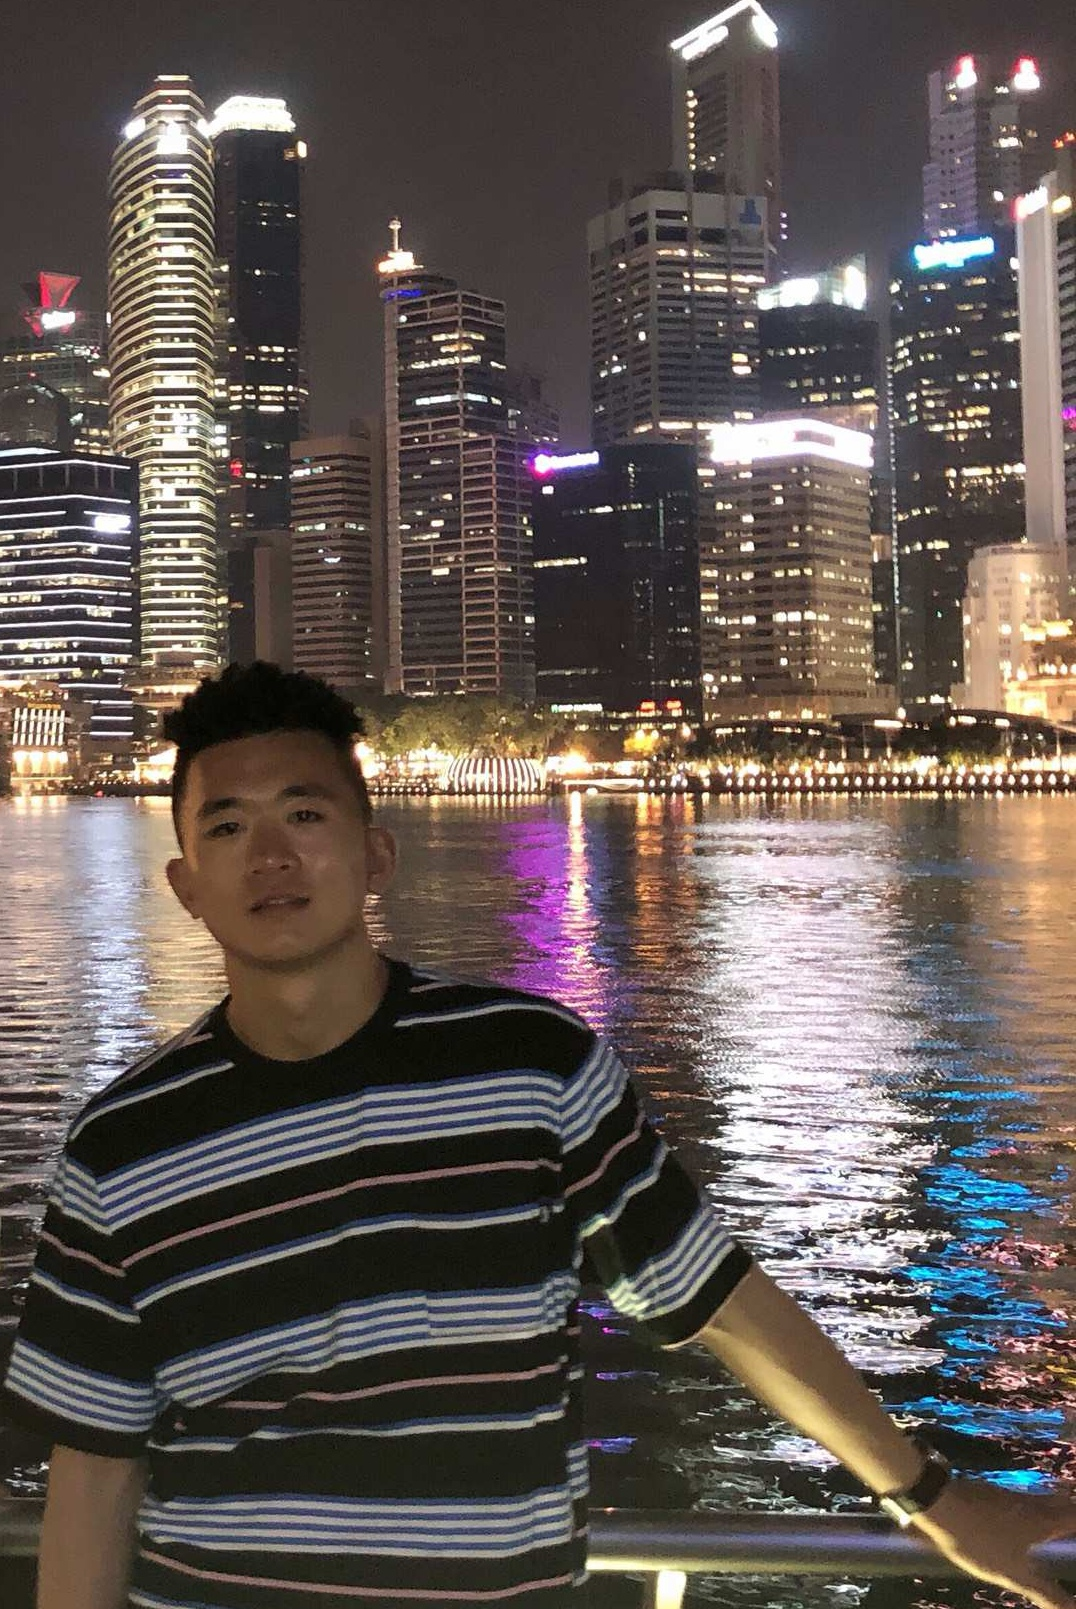
\includegraphics[height=3cm]{../people/hongyulu}
  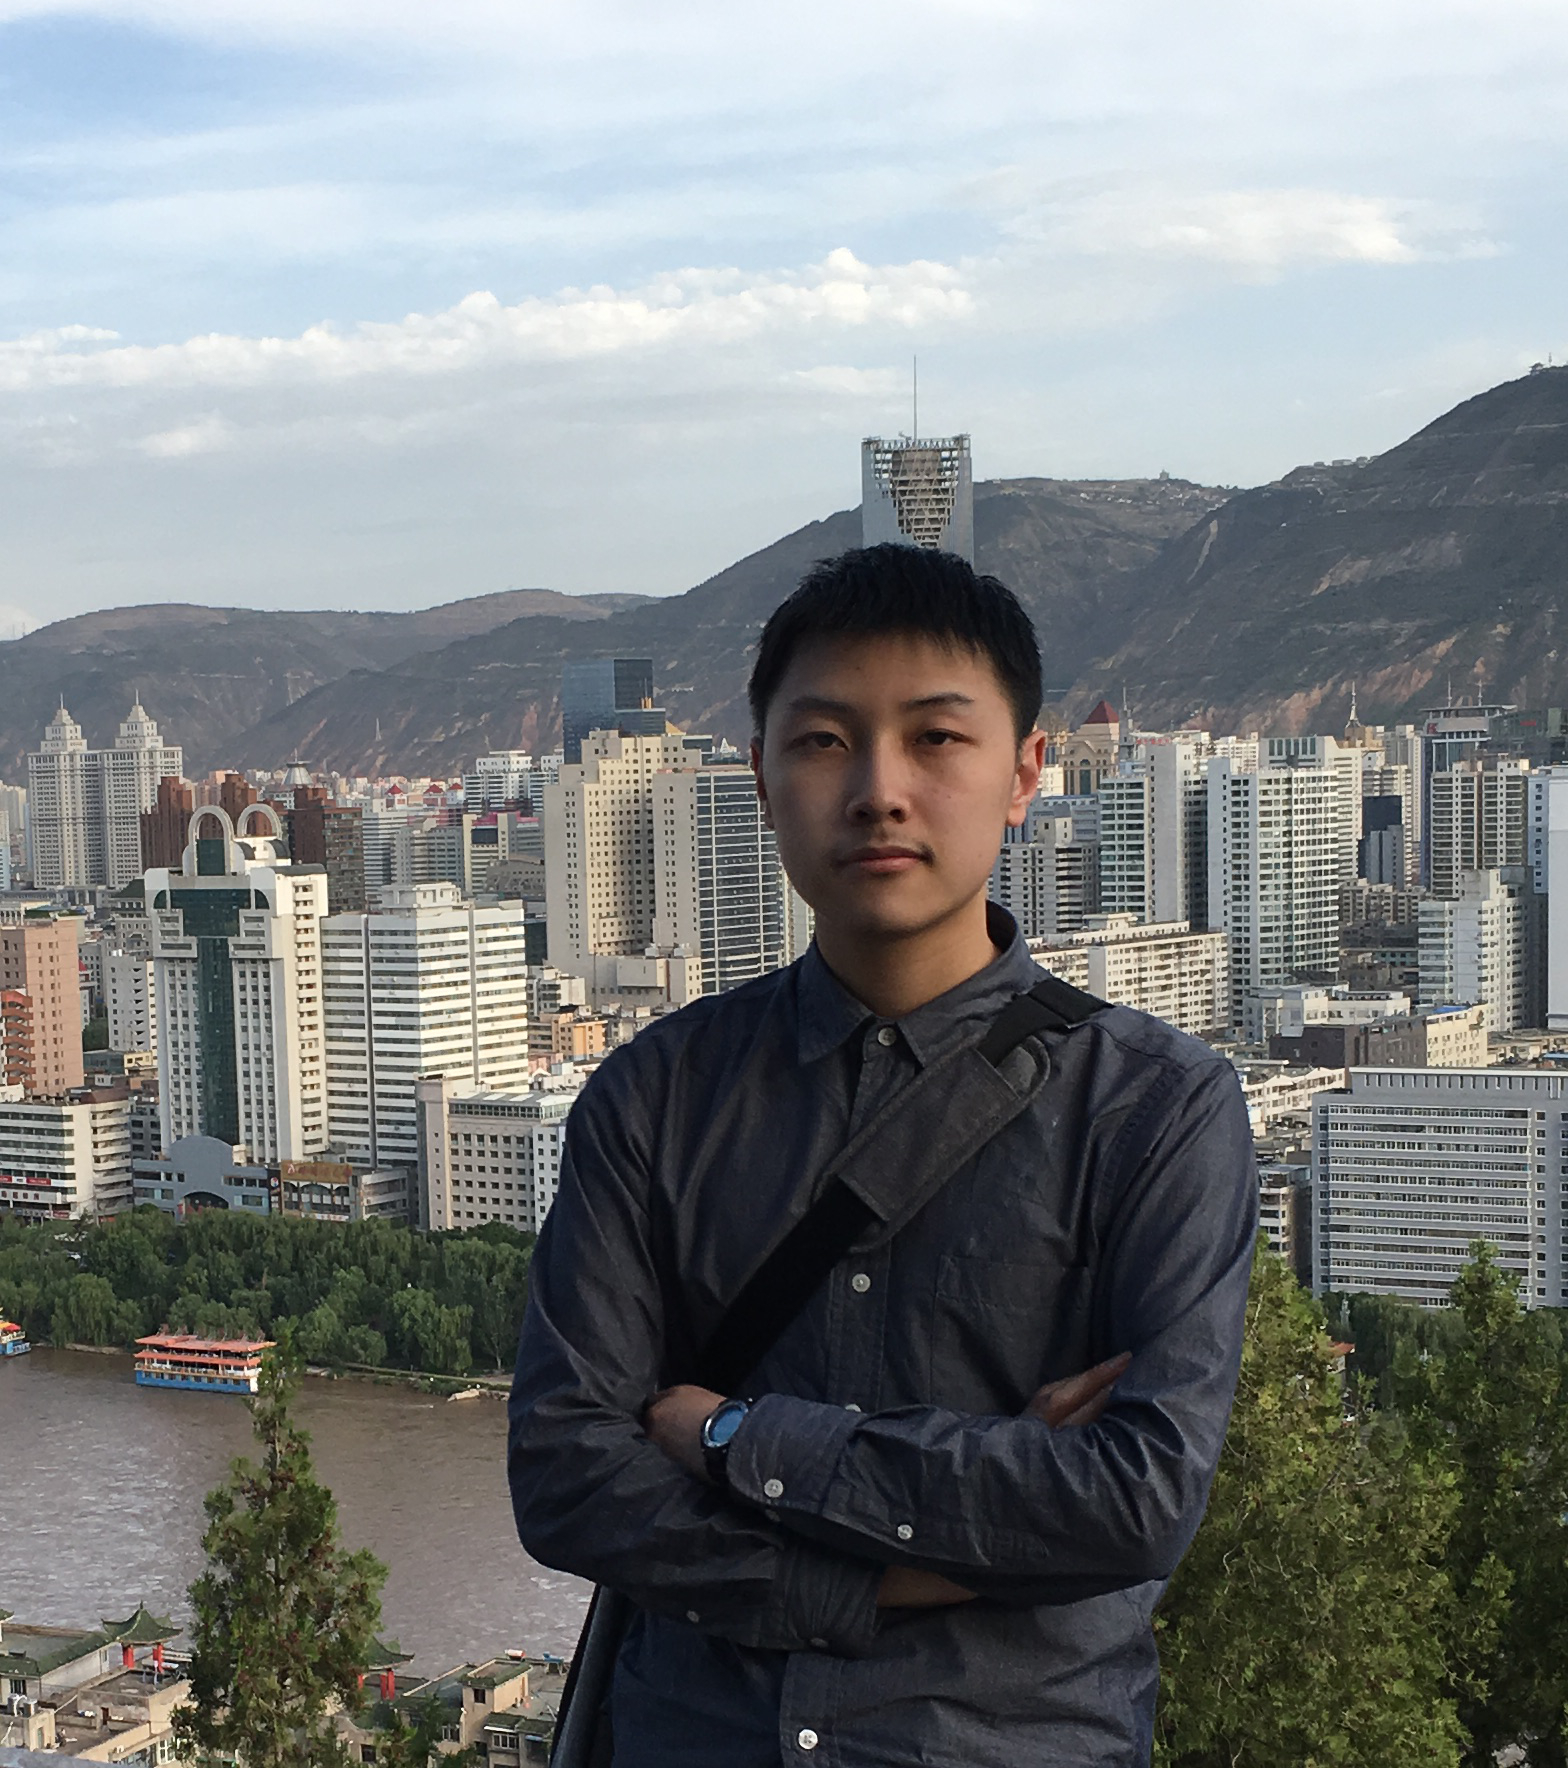
\includegraphics[height=3cm]{../people/chuhaoli}
  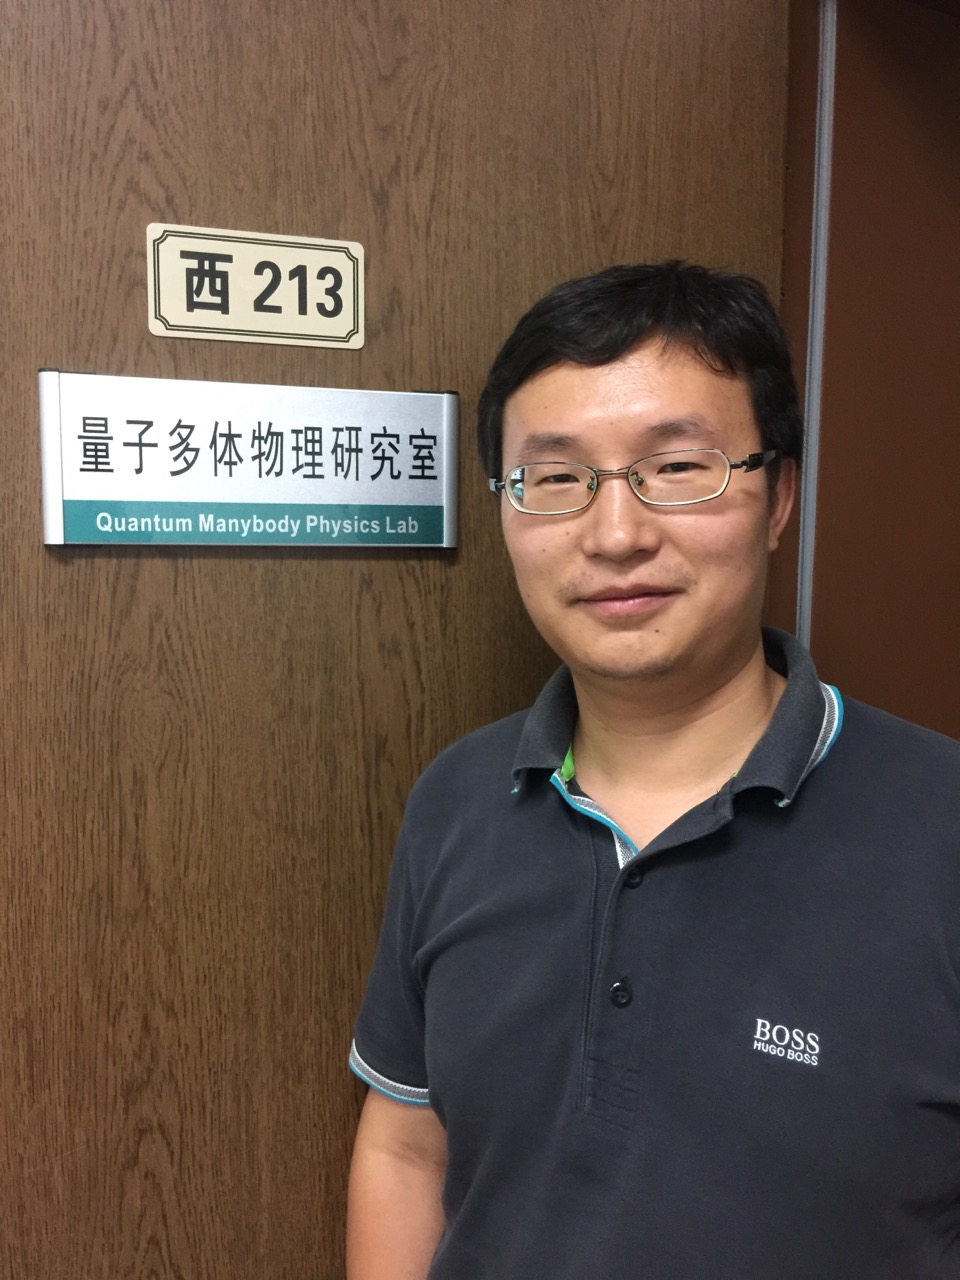
\includegraphics[height=3cm]{../people/weili}
  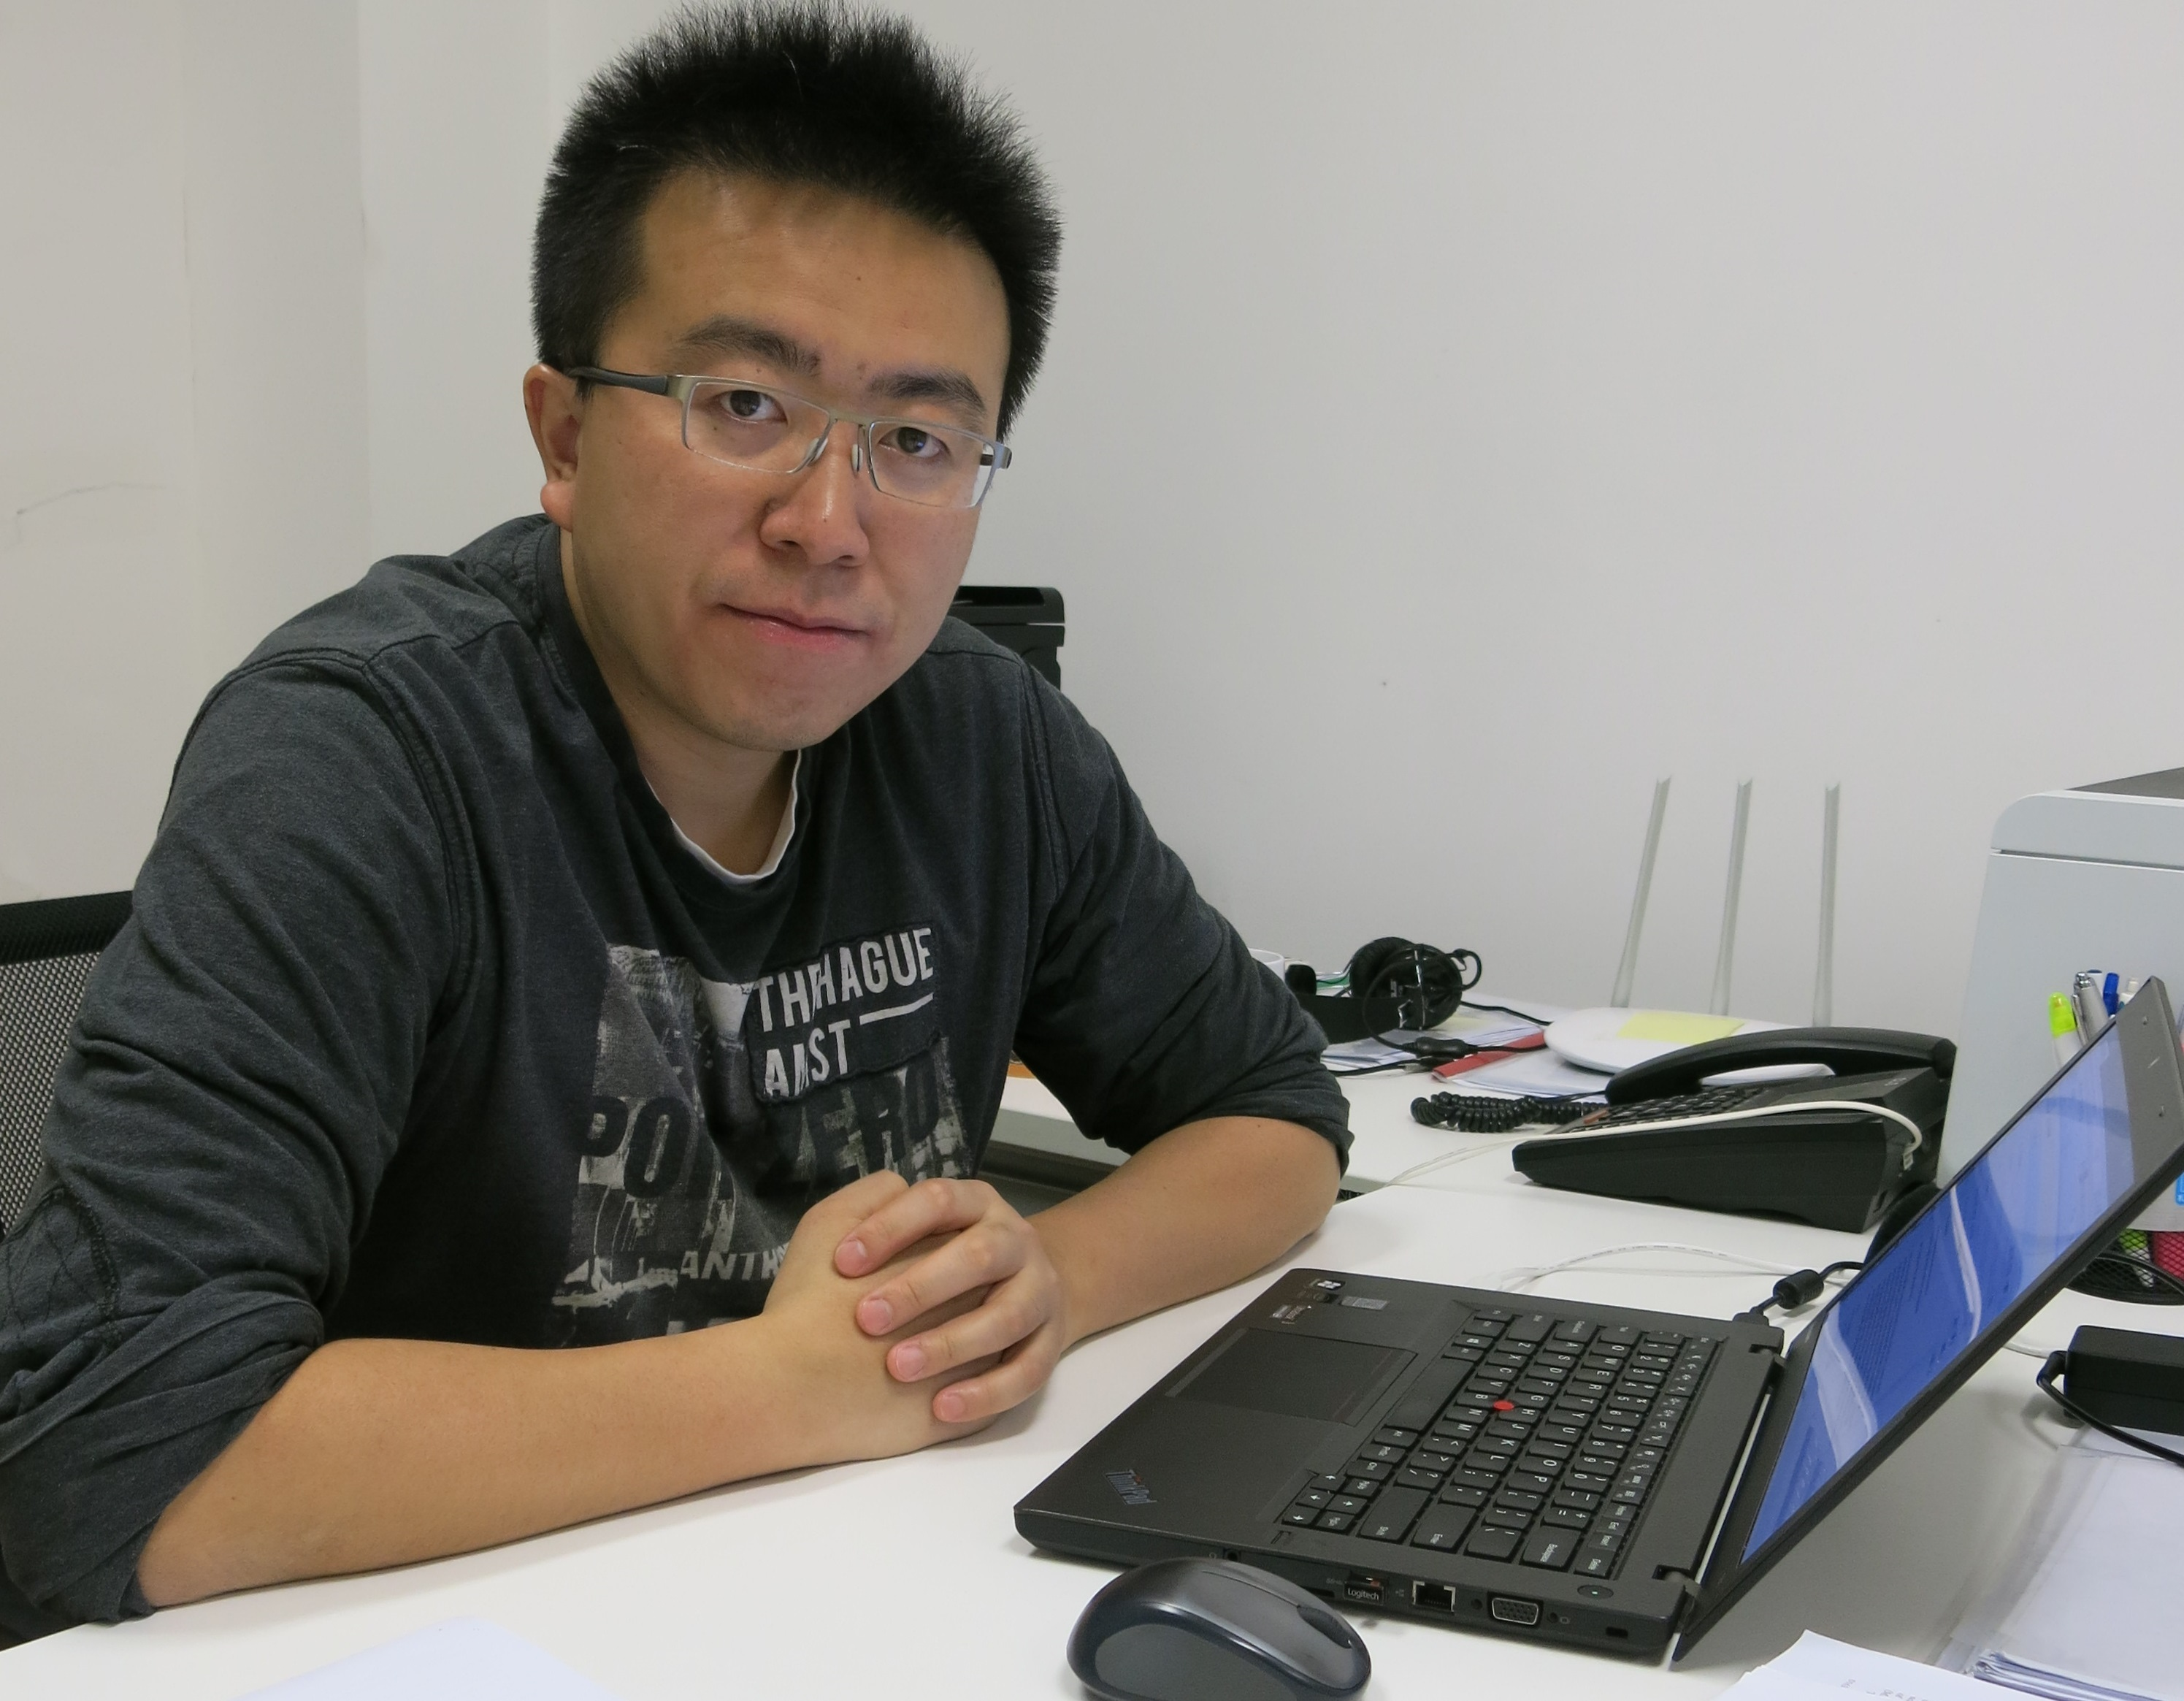
\includegraphics[height=3cm]{../people/ziyangmeng}
\end{center}
\end{itemize}
\end{frame}

\begin{frame}{Outline}
	%\begin{columns}
	%\column{.7\textwidth}
		\tableofcontents
  %\end{columns}
  % You might wish to add the option [pausesections]
\end{frame}

\section{Introduction to Monte Carlo Simulations: why we use a Markov Chain}

\begin{frame}
  \frametitle{Monte Carlo simulation: an unbiased method}
  \begin{itemize}
    \item A widely used numerical method in statistical physics and quantum many-body physics.
    \item Unbiased: reliable statistical error bar.
    \item Fast: polynomial complexity.
    \item Universal: applies to any model without the sign program.
  \end{itemize}
\end{frame}

\begin{frame}
  \frametitle{Introduction to MCMC}
  \begin{itemize}
    \item Consider a statistical mechanics model:
    \[Z=\sum_{\mathcal C}e^{-\beta H[\mathcal C]} = \sum_{\mathcal C}W(\mathcal C).\]
    \item The Markov-chain Monte Carlo (MCMC) is a way to do importance sampling.
    \item A Markov chain is constructed,
    \[\cdots\rightarrow\mathcal C_{i-1}\rightarrow\mathcal C_i\rightarrow\mathcal C_{i+1}\rightarrow\cdots\]
    \item Markov chain: $p(\mathcal C_i\rightarrow\mathcal C_j)$ only depends on $\mathcal C_i$ (no memory).
    \item Goal: distribution of $\mathcal C$ converges to the Boltzmann distribution $W(\mathcal C)$.
    \item Any observable can be measured from a Markov chain,
    \[\langle O\rangle = \frac{\sum O(\mathcal C)W(\mathcal C)}{\sum W(\mathcal C)} \simeq
     \frac1{\mathcal N}\sum_iO(\mathcal C_i).\]
    \item Quantum Monte Carlo: a quantum statistical model is mapped to a classical statistical model.
  \end{itemize}
\end{frame}

\begin{frame}
  \frametitle{Detailed balance}
  \begin{itemize}
    \item Detailed balance:
    \[\mathcal C\leftrightarrow\mathcal D,\quad
		\frac{p(\mathcal C\rightarrow\mathcal D)}{p(\mathcal D\rightarrow\mathcal C)}=\frac{W(\mathcal D)}{W(\mathcal C)}.\]
    \item Detailed balance (and ergodicity) guarantees that if the MC converges, it converges to the desired distribution $W(\mathcal C)$.
    \item Metropolis-Hastings algorithm: propose -- accept/reject.
  \end{itemize}
\begin{columns}
\column{.5\textwidth}
\begin{tikzpicture}
\node at (0, 0) (C) [draw,circle] {$\mathcal C$};
\node<2-> at (3, 0) (D) [draw, rectangle] {$\mathcal D?$};
\node<2-> at (3, 1.5) (D1) [draw, rectangle] {$\mathcal D_1?$};
\node<2-> at (3, -1.5) (D2) [draw, rectangle] {$\mathcal D_2?$};
\node<2-> at (3, -2) {$\vdots$};
\draw<2-> [->] (C)--(D) node [midway, above] {{\small $q(\mathcal C\rightarrow\mathcal D)$}};
\draw<2-> [->] (C)--(D1);
\draw<2-> [->] (C)--(D2);
\node<3-> at (6, 1) (DD) [draw, circle] {$\mathcal D$};
\node<3-> at (6, -1) (DC) [draw, circle] {$\mathcal C$};
\draw<3-> [->] (D)--(DD) node [midway, above] {{\small $\alpha(\mathcal C\rightarrow\mathcal D)$}};
\draw<3-> [->] (D)--(DC);
\end{tikzpicture}
\column{.5\textwidth}
\begin{block}{Steps of Metropolis-Hastings algorithm}
\begin{enumerate}
\item<2-> Select a new state $\mathcal D_i$.
\item<3-> Accept or reject.
    \[p(\mathcal C\rightarrow\mathcal D) = q(\mathcal C\rightarrow\mathcal D)
    \alpha(\mathcal C\rightarrow\mathcal D).\]
    \[\alpha(\mathcal C\rightarrow\mathcal D) =
    \min\left\{1, \frac{W(\mathcal D)}{W(\mathcal C)}
    \frac{q(\mathcal D\rightarrow\mathcal C)}
    {q(\mathcal C\rightarrow\mathcal D)}\right\}.\]
\end{enumerate}
\end{block}
\end{columns}
\end{frame}

\begin{frame}
  \frametitle{Autocorrelation time}
  \begin{itemize}
    \item Autocorrelation time measures the efficiency of the update algorithm.
    \item ``time'' sequence:
    \[\cdots\rightarrow O(t-1)\rightarrow O(t)\rightarrow O(t+1)\rightarrow\cdots,
  \quad O(t) = O[\mathcal C(t)].\]
    \item Autocorrelation function
    \[\mathcal A_O(\Delta t)=\langle O(t)O(t+\Delta t)\rangle - \langle O(t)\rangle^2\propto e^{-\Delta t/\tau}.\]
  \end{itemize}
  \begin{columns}
    \column{.7\textwidth}
    \begin{block}{Complexity $\propto \tau$}
      \[\langle O\rangle = \frac1{\mathcal N}\sum_iO(\mathcal C_i).\]
      Statistical error $\delta O\sim\frac1{\sqrt{\mathcal N}}$ only if $O(i)$ are independent.

A statistically independent sample is generated in every $\tau$-steps.
\[\text{Complexity}=\text{Complexity of each step}\times\tau\times\mathcal N.\]
    \end{block}
    \column{.3\textwidth}
    \centering
    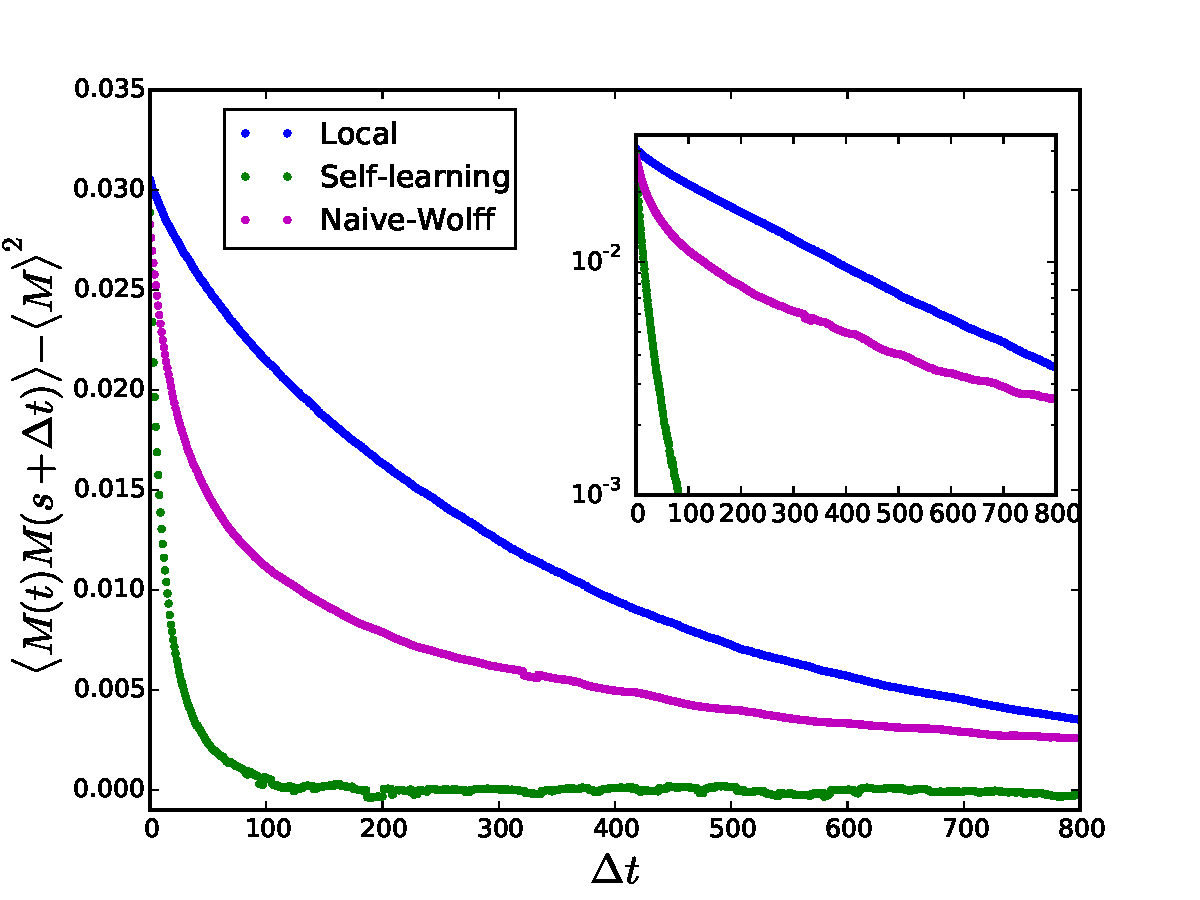
\includegraphics[height=3.5cm]{../slmctut/auto_decay}
  \end{columns}
\end{frame}

\begin{frame}
  \frametitle{Performence of the algorithm}
    \begin{columns}
			\column{.5\textwidth}
      \begin{center}
				Theory\\
				\vspace{.5cm}
        
\includegraphics[height=4cm]{../slmctut/laptop_coffee}
      \end{center}
			\column{.5\textwidth}
      \begin{center}
				Reality\\
				\vspace{.5cm}
        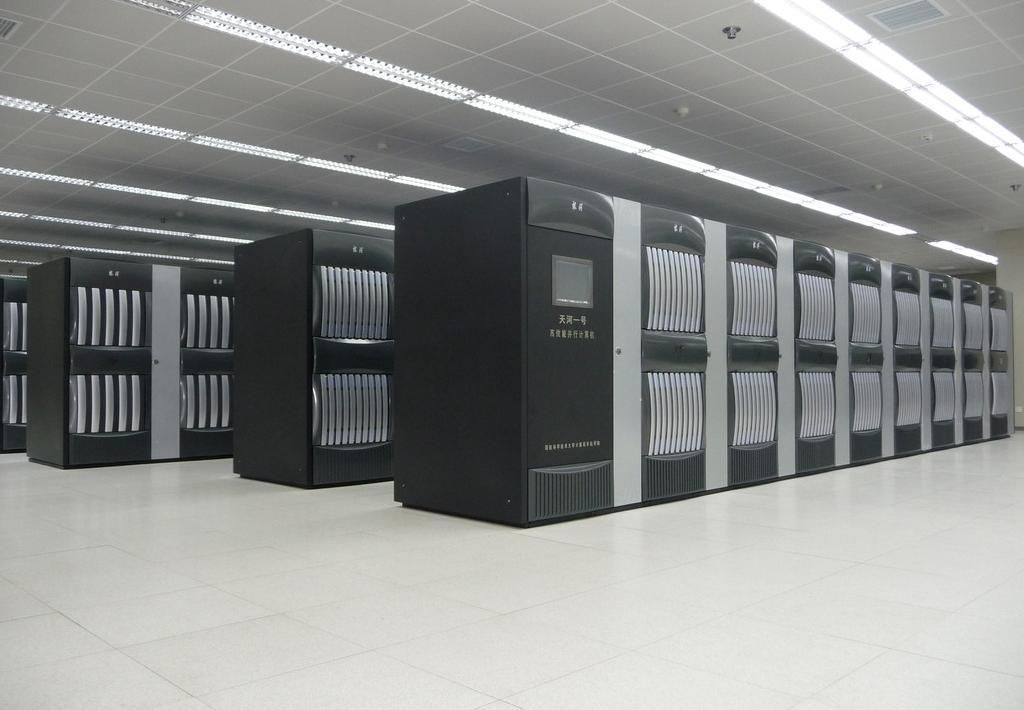
\includegraphics[height=4cm]{../slmctut/tianhe}
      \end{center}
      %\item Why?
      %\[\text{Cost} \propto \text{Cost of each step} \times \text{autocorrelation time}\]
    \end{columns}
\vspace{.5cm}
Most of our simulation is done on the Tianhe-1 supercomputer in Tianjin, China.
\end{frame}

\begin{frame}
  \frametitle{A good update samples low-energy states}
  \begin{center}
    \begin{tikzpicture}
      \draw plot[domain=0:9.52,smooth,samples=200] function {sin(x*2)};
      \draw<1> (2.356, -1) -- (2.8, -0.63127) [->, thick];
      \draw<2> (2.356, -1) -- (3.5, 0.65699) [->, thick];
      \draw<3> (2.356, -1) -- (5.49779, -1) [->, thick];
    \end{tikzpicture}
  \end{center}
  \begin{itemize}
    \item A dilemma of local updates:
    \item<1-> Step is too small: high acceptance, small difference.
    \item<2-> Step is too big: low acceptance, big difference.
  \end{itemize}
\end{frame}

\begin{frame}
  \frametitle{Local Update: Metropolis algorithm}
  \begin{center}
    \begin{tikzpicture}
      \node at (0, 0) [circle, draw] {};
      \node at (1, 0) [circle, draw] {};
      \node at (0, 1) [circle, draw] {};
      \node at (-1, 0) [circle, fill, draw] {};
      \node at (0, -1) [circle, fill, draw] {};

      \node at (4, 0) [circle, fill, draw] {};
      \node at (5, 0) [circle, draw] {};
      \node at (4, 1) [circle, draw] {};
      \node at (3, 0) [circle, fill, draw] {};
      \node at (4, -1) [circle, fill, draw] {};

      \draw [<->, thick] (1.5, 0)--(2.5, 0);
    \end{tikzpicture}
  \end{center}
  \begin{itemize}
    \item Consider the Ising model.
    \item Local update: randomly select a site and flip the spin.
    \item $q(\mathcal C\rightarrow\mathcal D) = q(\mathcal D\rightarrow\mathcal C) = \frac1N$.
    \item $\alpha(\mathcal C\rightarrow\mathcal D)=\min\left\{1,\frac{W(\mathcal D)}{W(\mathcal C)}\right\}.$
    \item $N$ trials are counted as one MC step.
    \item Very general: applies to any model.
    \item N Metropolis, A W Rosenbluth, M N Rosenbluth, A H Teller, and E Teller, J Chem Phys \textbf{21}, 1087 (1953).
  \end{itemize}
\end{frame}

\begin{frame}
  \frametitle{Critical slowing down}
  \begin{itemize}
    \item The real dynamical relaxation time diverges at the critical point: a critical system is slow to equilibrate.
    \item The local update mimics the real relaxation process: also exhibits the critical slowing down phenomena.
    \item $\tau\propto L^z$, $z=2.125$ for the 2D Ising model.
  \end{itemize}
  \begin{center}
    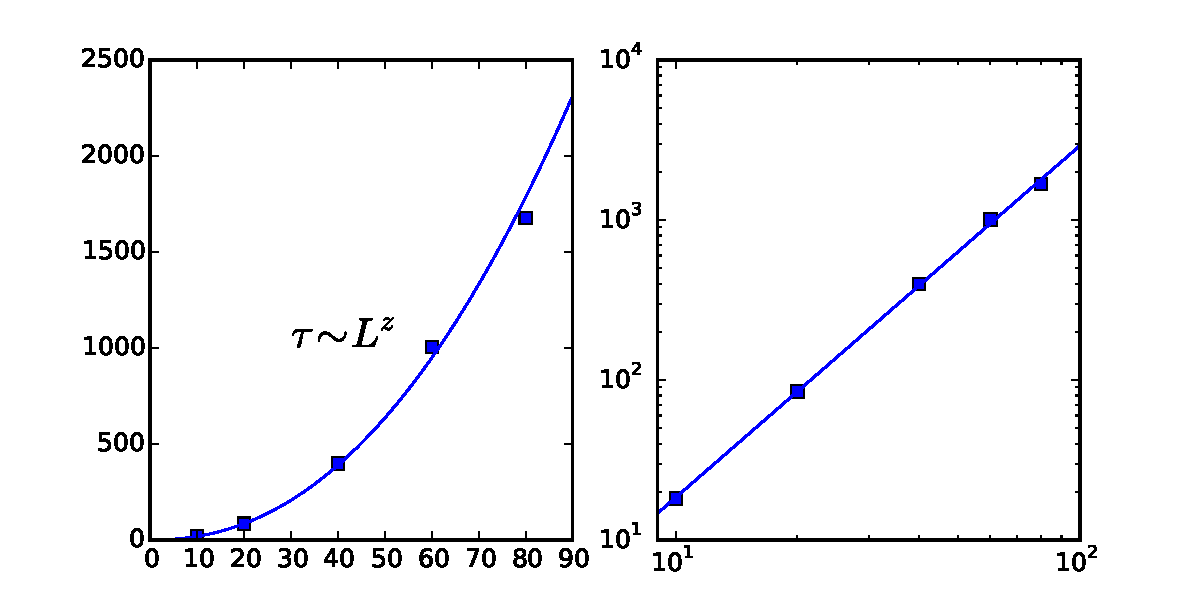
\includegraphics[width=8cm]{../slmctut/slowdown}
  \end{center}
  There's a way around this: MCMC simulation does not have to mimic the real dynamics...
\end{frame}

\begin{frame}
  \frametitle{Challenge}
  \begin{itemize}
    \item Local update is too slow for many models: critical slowing down, glassy behavior, separation of energy scales, etc.
    \item Global update is only available for certain models. Like Wolff algorithm for two-body interactions.
    \item A good update algorithm for generic models?
  \end{itemize}
\end{frame}

\section{Direct Sampling: Generative Model + a short Markov chain}

\begin{frame}
  \frametitle{Generative model}
  \begin{itemize}
  \item NN transforms Gaussian variables to target distribution.
  \item PBC padding before convolutional layers.
  \item Continuous input, 0/1 output.
  \end{itemize}
  \begin{center}
    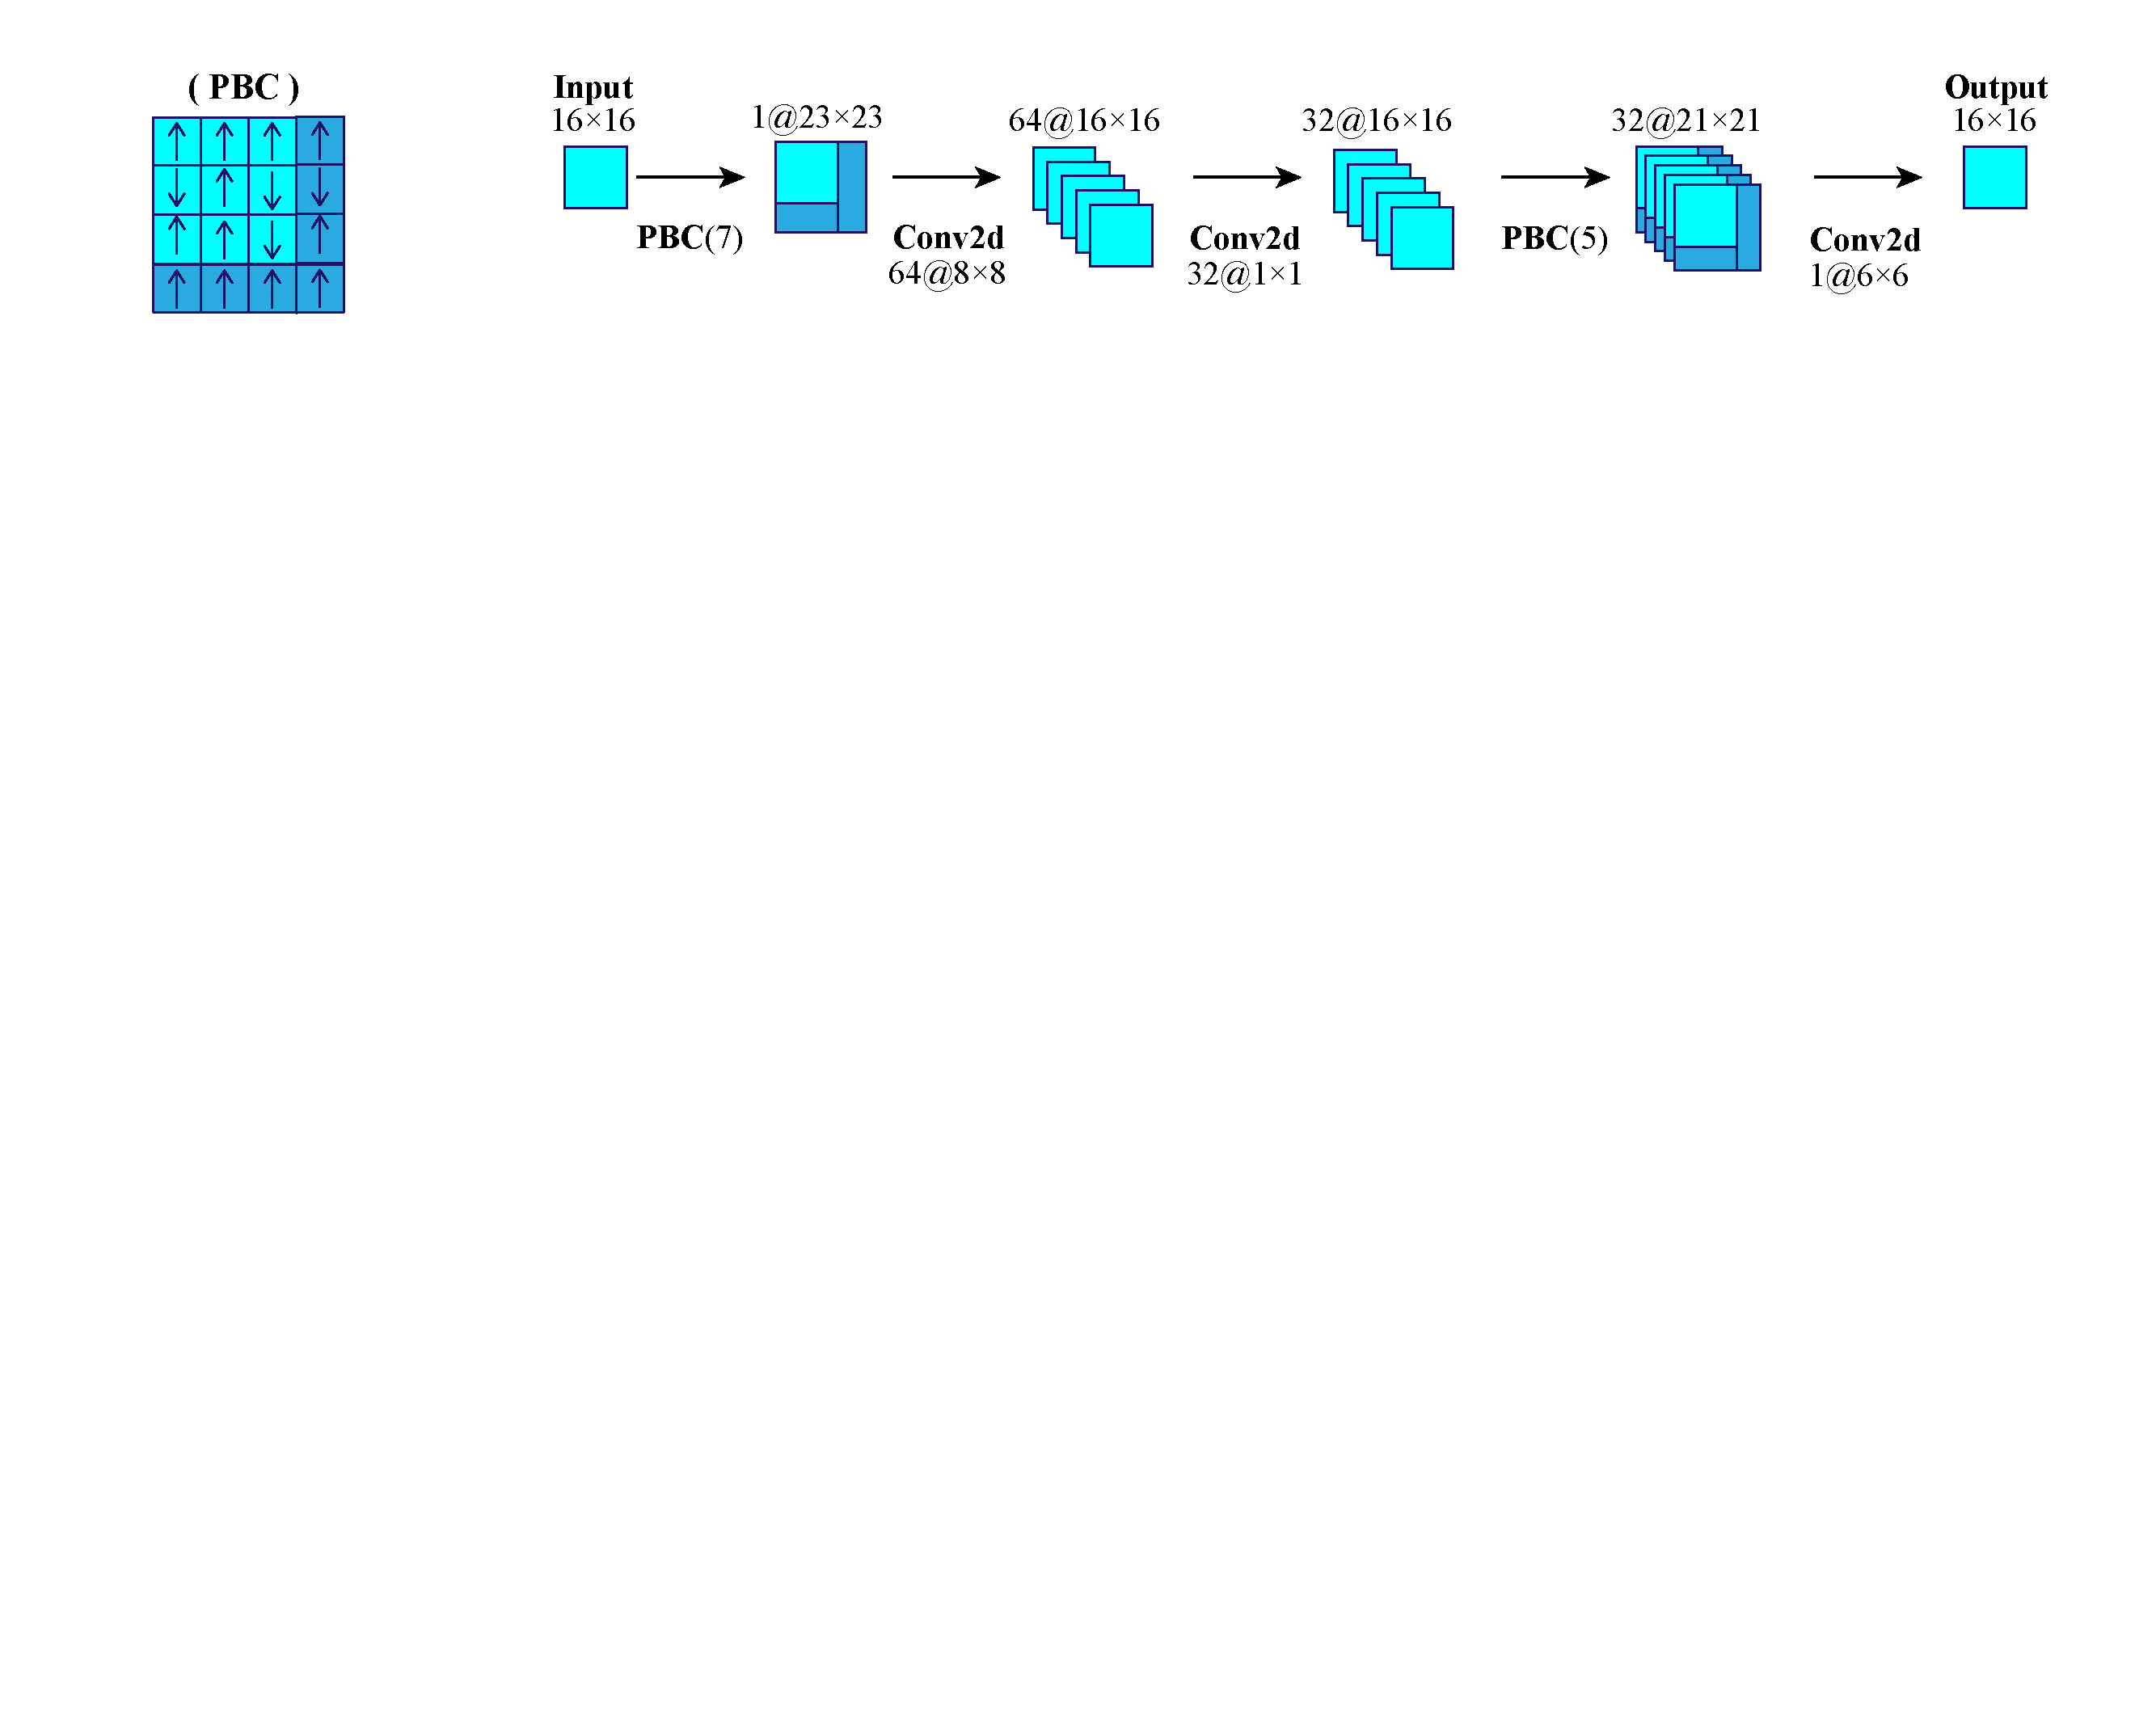
\includegraphics[width=14cm]{nn-model1}
  \end{center}
\end{frame}

\begin{frame}
  \frametitle{Training the model}
  \begin{itemize}
  \item Training sample generated by an MCMC simulation.
  \item Criterion: the NN distribution and the training set produces the same physical observables.\\
    Energy, spin-spin correlation, etc.
  \item Loss function:
    \begin{align*}
      \text{Loss}(\{G_i\},\{C_i\})=&w_1\sum_i[|M|(\{G_i\})-|M|(\{C_i\})]^2\\
      &+w_2 [M^2(\{G_i\})-M^2(\{C_i\})]^2+w_3 [E(\{G_i\})-E(\{C_i\})]^2
    \end{align*}

  \end{itemize}
\end{frame}

\begin{frame}
  \frametitle{Advantage of the generative model: no autocorrelation}
  Direct sampling on the generative model:
  \begin{itemize}
  \item Fast sampling.
  \item No autocorrlation.
  \end{itemize}
  \begin{center}
    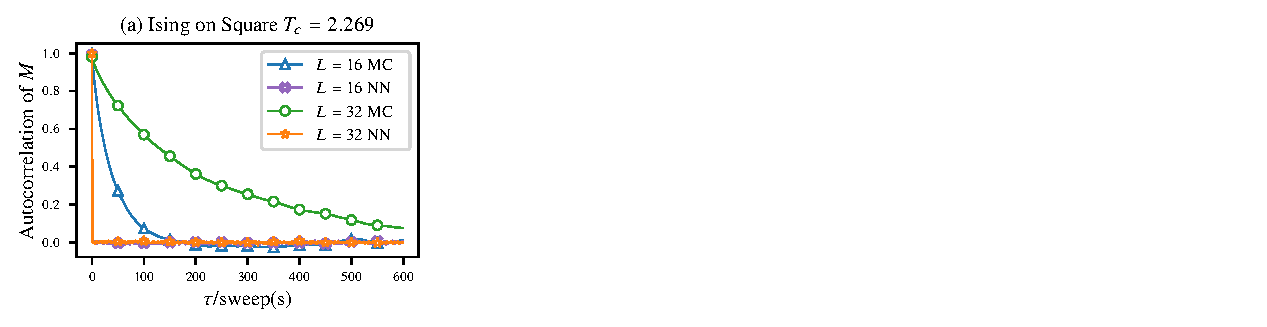
\includegraphics{autocorr-a}
  \end{center}
\end{frame}

\begin{frame}
	\frametitle{Limitation of the generative model}
	\begin{itemize}
		\item The training sample is inaccurate: We do this because MCMC is not good enough...
		\item The generative model learns all inaccurate details of the training sample.
		\item The generative model cannot supercede the accuracy of the training sample.
	\end{itemize}
\end{frame}

\begin{frame}
  \frametitle{Correcting the generative model with a short Markov chain}
	\begin{itemize}
		\item The generative model is close to the true distribution.
		\item Start from the generative model, a few MCMC steps coverge to the true distribution.
		\item A non-MC direct sampling:
		\begin{center}
			\begin{tikzpicture}
				\draw (0,0) node (n1) [draw] {NN};
				\draw (1.5,0) node (m11) [circle,draw] {MC};
				\draw (3,0) node (m12) [circle,draw] {MC};
				\draw [->] (n1) -- (m11);
				\draw [->] (m11)--(m12);

				\draw (4.5,0) node (n2) [draw] {NN};
				\draw (6,0) node (m21) [circle,draw] {MC};
				\draw (7.5,0) node (m22) [circle,draw] {MC};
				\draw [->] (n2) -- (m21);
				\draw [->] (m21)--(m22);

				\draw (9,0) node (n2) [draw] {NN};
				\draw (10.5,0) node (m21) [circle,draw] {MC};
				\draw (12,0) node (m22) [circle,draw] {MC};
				\draw [->] (n2) -- (m21);
				\draw [->] (m21)--(m22);
			\end{tikzpicture}
		\end{center}
	\end{itemize}
\end{frame}

\begin{frame}
  \frametitle{Correcting the generative model with a short Markov chain}
	\begin{columns}
		\column{.7\textwidth}
		\begin{center}
			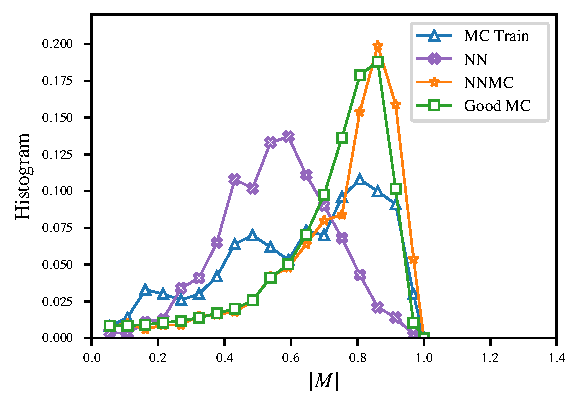
\includegraphics[height=7cm]{hist-ising}
		\end{center}
		\column{.3\textwidth}
		\begin{itemize}
			\item Training data has a wrong distribution.
			\item NN learns the wrong dist.
			\item NN + short MC recovers the correct dist.
		\end{itemize}
	\end{columns}
\end{frame}
\section{Application to quantum fermionic systems}

\begin{frame}
	\frametitle{Converting fermionic quantum models to classical models}
	\begin{itemize}
		\item Auxiliary-field determinant quantum Monte Carlo (AFDQMC).
		\item Configurations: space-time configuration of classical auxiliary fields.
		\item Weights: $W[\{S_i\}] = \det (1 + B[\{S_i\}])$.
		\item Effective bosonic model with nonlocal interactions: can a CNN model express this?
	\end{itemize}
	\begin{center}
		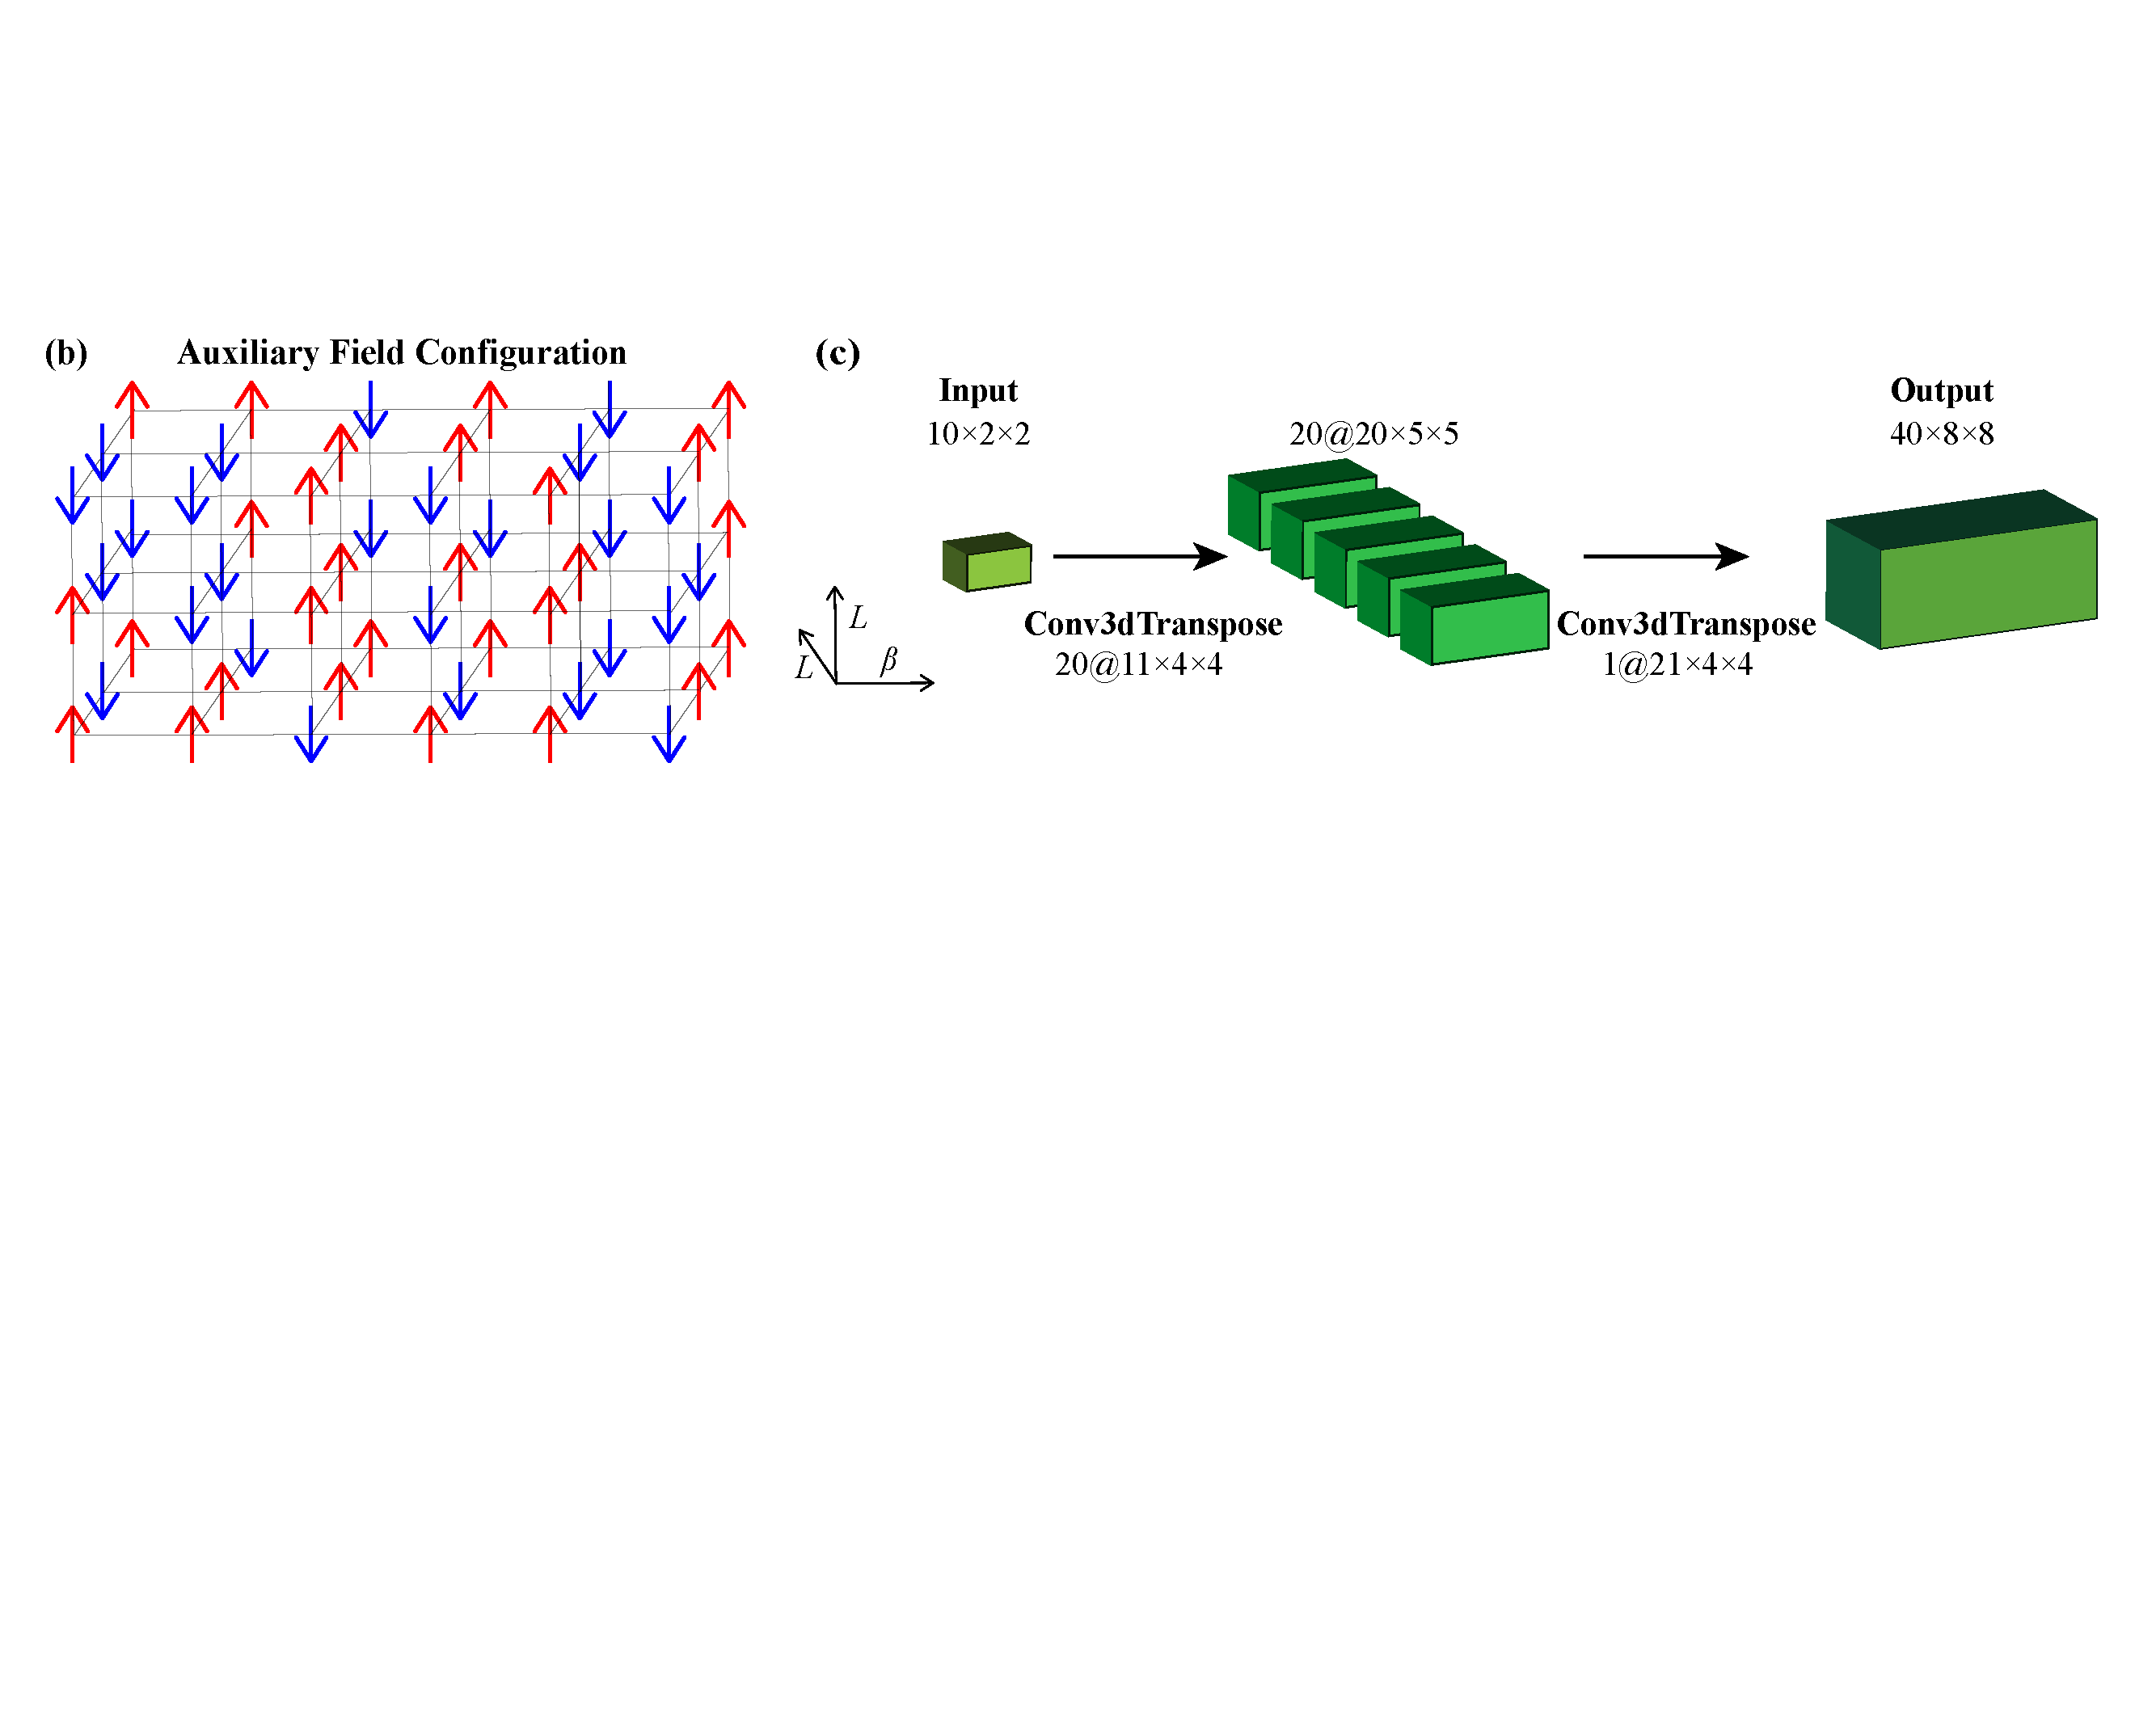
\includegraphics[height=3cm]{nn-model2}
	\end{center}
\end{frame}

\begin{frame}
	\frametitle{Results}
	\begin{columns}
		\column{.5\textwidth}
		\begin{center}
			Direct sampling
			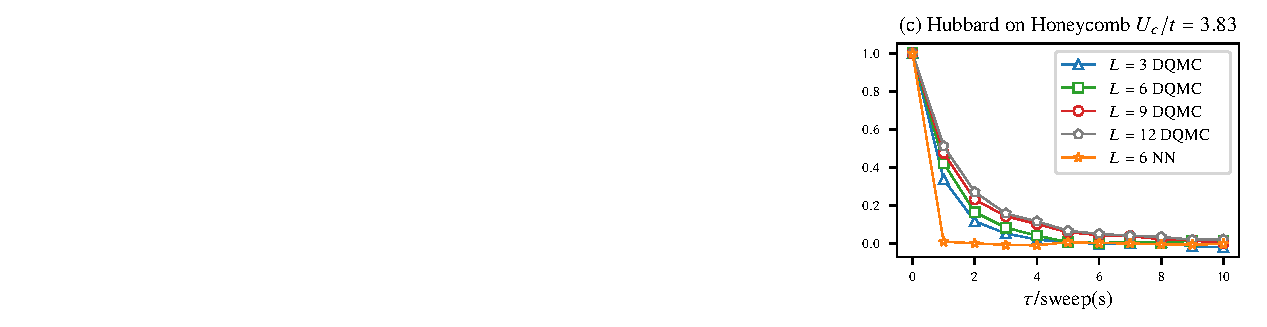
\includegraphics{autocorr-c}
		\end{center}
		\column{.5\textwidth}
		\begin{center}
			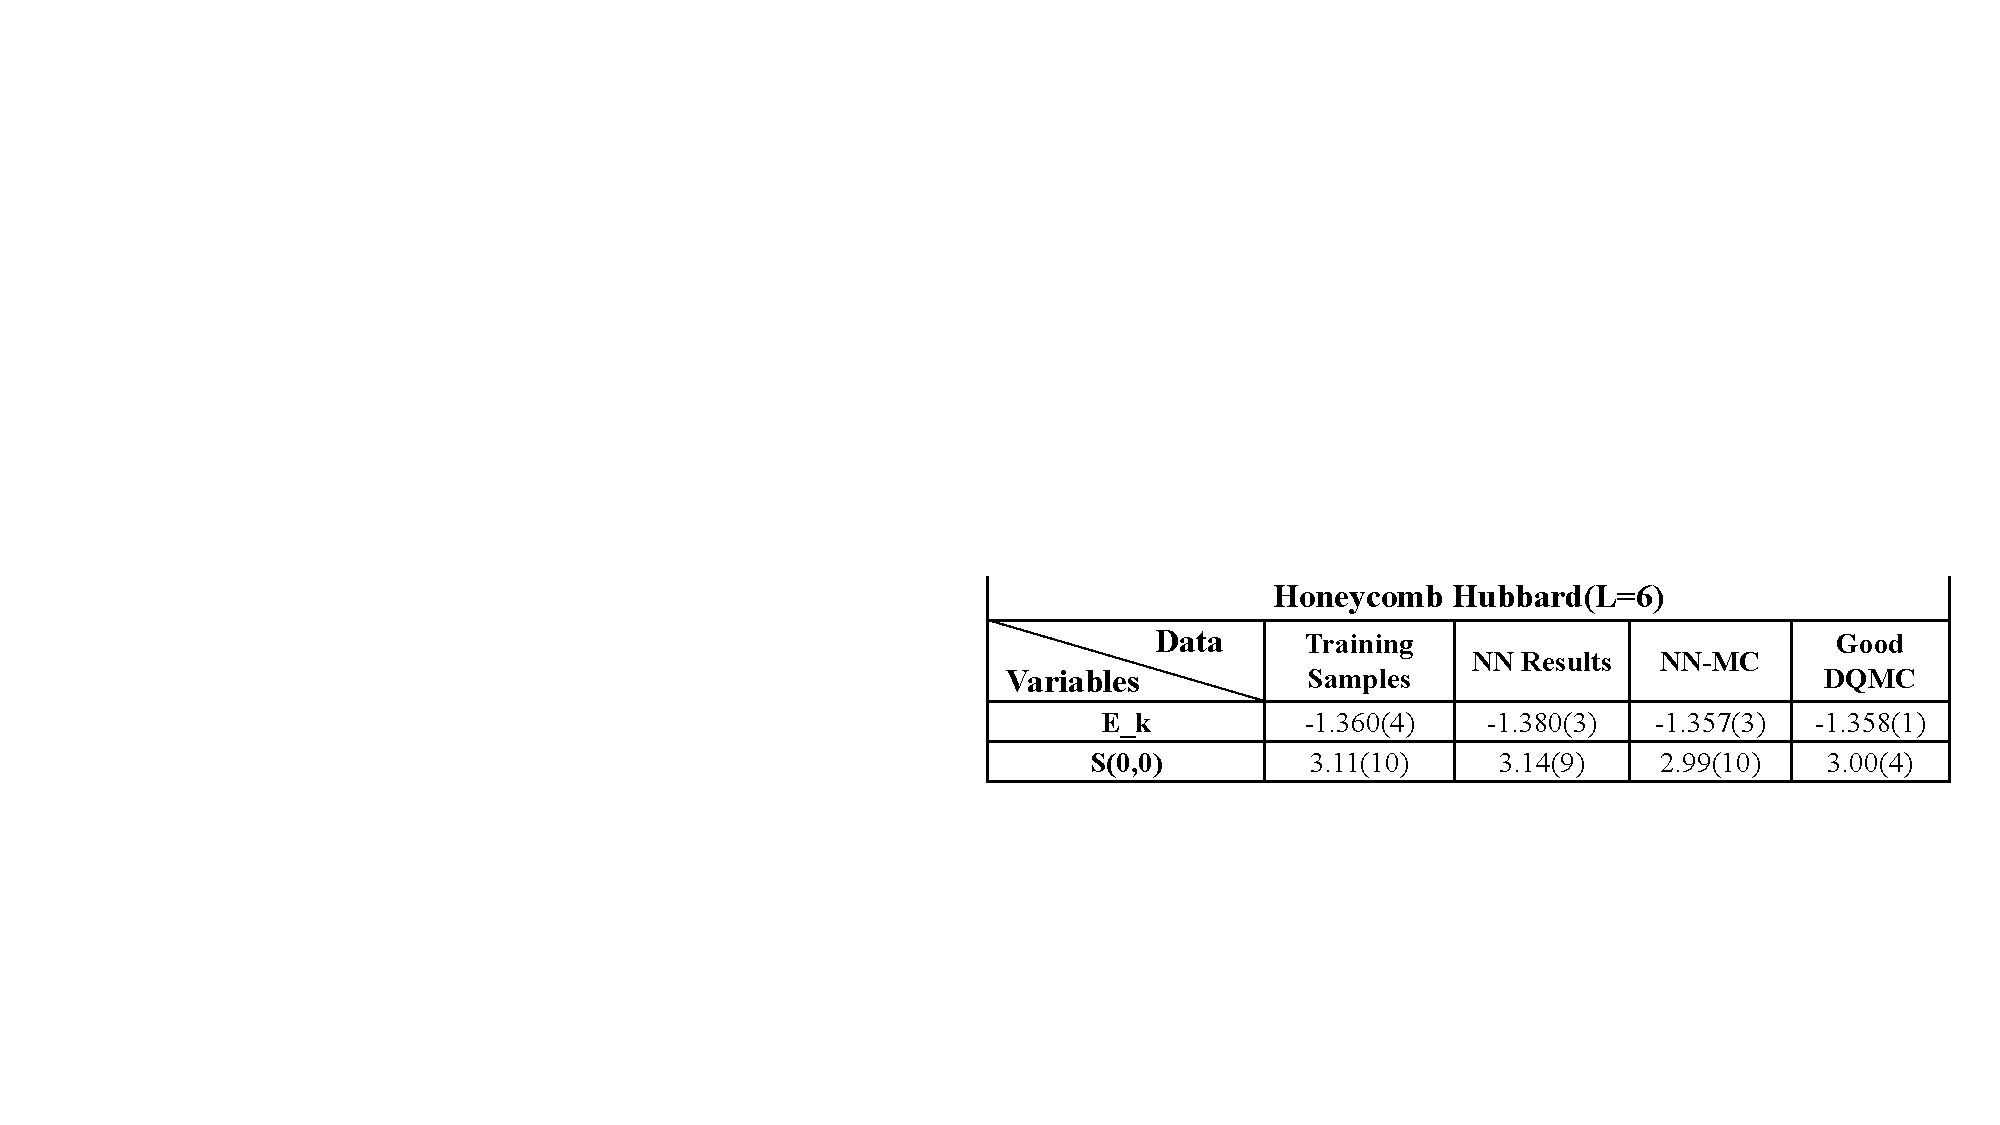
\includegraphics[width=7cm]{corr-2}
		\end{center}

	\end{columns}
\end{frame}

\section{Details and Conclusions}


\end{document}
